\documentclass[handout, 12pt]{beamer}
\usetheme{focus}

\setbeamertemplate{caption}[numbered]
\usepackage{booktabs, multirow, array}
\usepackage{CJKutf8}
\usepackage{pifont}
\newcommand{\xmark}{\ding{55}}
\usepackage{dirtree}
\setlength{\DTbaselineskip}{10pt}
\DTsetlength{0.2em}{1em}{0.2em}{0.4pt}{0pt}
\renewcommand*\DTstylecomment{\sffamily}

\usepackage{svg}
\usepackage{fontawesome5}

%\usepackage[fontset=windows]{ctex}
\usepackage{xcolor}
\definecolor{amaranth}{rgb}{0.9, 0.17, 0.31}
\definecolor{ballblue}{rgb}{0.13, 0.67, 0.8}

\usepackage{listings}
\definecolor{codecomment}{RGB}{36, 128, 103}
\definecolor{codekeyword}{RGB}{238, 63, 77}
\definecolor{codestring}{RGB}{19, 72, 87}
\lstdefinestyle{mystyle}{
	commentstyle=\color{codecomment},
	keywordstyle=\color{codekeyword},
	stringstyle=\color{codestring},
	numberstyle=\tiny\color{main},
	basicstyle=\ttfamily\scriptsize,
	numbersep=5pt,
	tabsize=4,  % 設定 Tab 轉換為 4 個空格
	keepspaces=true,  % 確保空格與縮排不會被改變
	columns=fixed,    % 強制固定列寬，避免 Tab 出現 ^^I
	showspaces=false,
	showstringspaces=false,
	showtabs=false,   % 確保不顯示 Tab
}
\lstset{style=mystyle}

\usepackage{tikz, pgfplotstable}
\usepackage{pgfplots}
\pgfplotsset{compat=1.18}
\usetikzlibrary{arrows.meta}
\usepgfplotslibrary{dateplot}
\usetikzlibrary{decorations.pathreplacing,calligraphy}

\newcommand{\sol}{%
	\fcolorbox{white}{main}{\color{white}\,sol\,}%
}

\renewcommand{\baselinestretch}{1.35}

\usepackage{graphicx, float}
\graphicspath{{figures/}}  % 設定圖片預設資料夾

\usepackage{ragged2e}

\usepackage{tabularx}

\usepackage{algorithm2e}
\usepackage{amsmath}
\usepackage{animate}


\title{\fontsize{25}{20}\selectfont Report Generator}
\subtitle{\large Automated Document Creation with Flask}
\author{Anthony Sung}
\institute{National Chengchi University\vspace{-2em}}
\date{May 26, 2025}

\begin{document}
	\justifying
    \begin{frame}
        \maketitle
    \end{frame}

    \begin{frame}{Table of Contents}
        \tableofcontents
    \end{frame}
    
    \section{Introduction}

	\begin{frame}{Challenges in Manual Report Generation}
		\begin{columns}
			\begin{column}{.65\textwidth}
				\begin{itemize}
					\item Time-consuming, tedious, and repetitive
					\item Often leads to human-error
					\item \href{https://www.microsoft.com/en-us/power-platform/products/power-bi}{Power BI}, \href{https://www.tableau.com/}{Tableau}, or \href{https://www.fanruan.com/en/finereport}{FineReport}
				\end{itemize}
			\end{column}

			\begin{column}{.35\textwidth}
				\begin{figure}[H]
					\centering
					
\includegraphics[width=.9\textwidth]{time-consuming.pdf}
					\caption{Tired Man}
				\end{figure}
			\end{column}
		\end{columns}
	\end{frame}

	\begin{frame}{Why We Built This}
		\begin{itemize}
			\item One tool for templates, data, and automation
			\item Less coding needed --- just upload and go
			\item Built to work with \textbf{Google Drive} and charts
		\end{itemize}
	\end{frame}

	\begin{frame}{Smarter Reports, Less Effort}
		\begin{columns}
			\begin{column}{.35\textwidth}
				\begin{figure}[H]
					\centering
					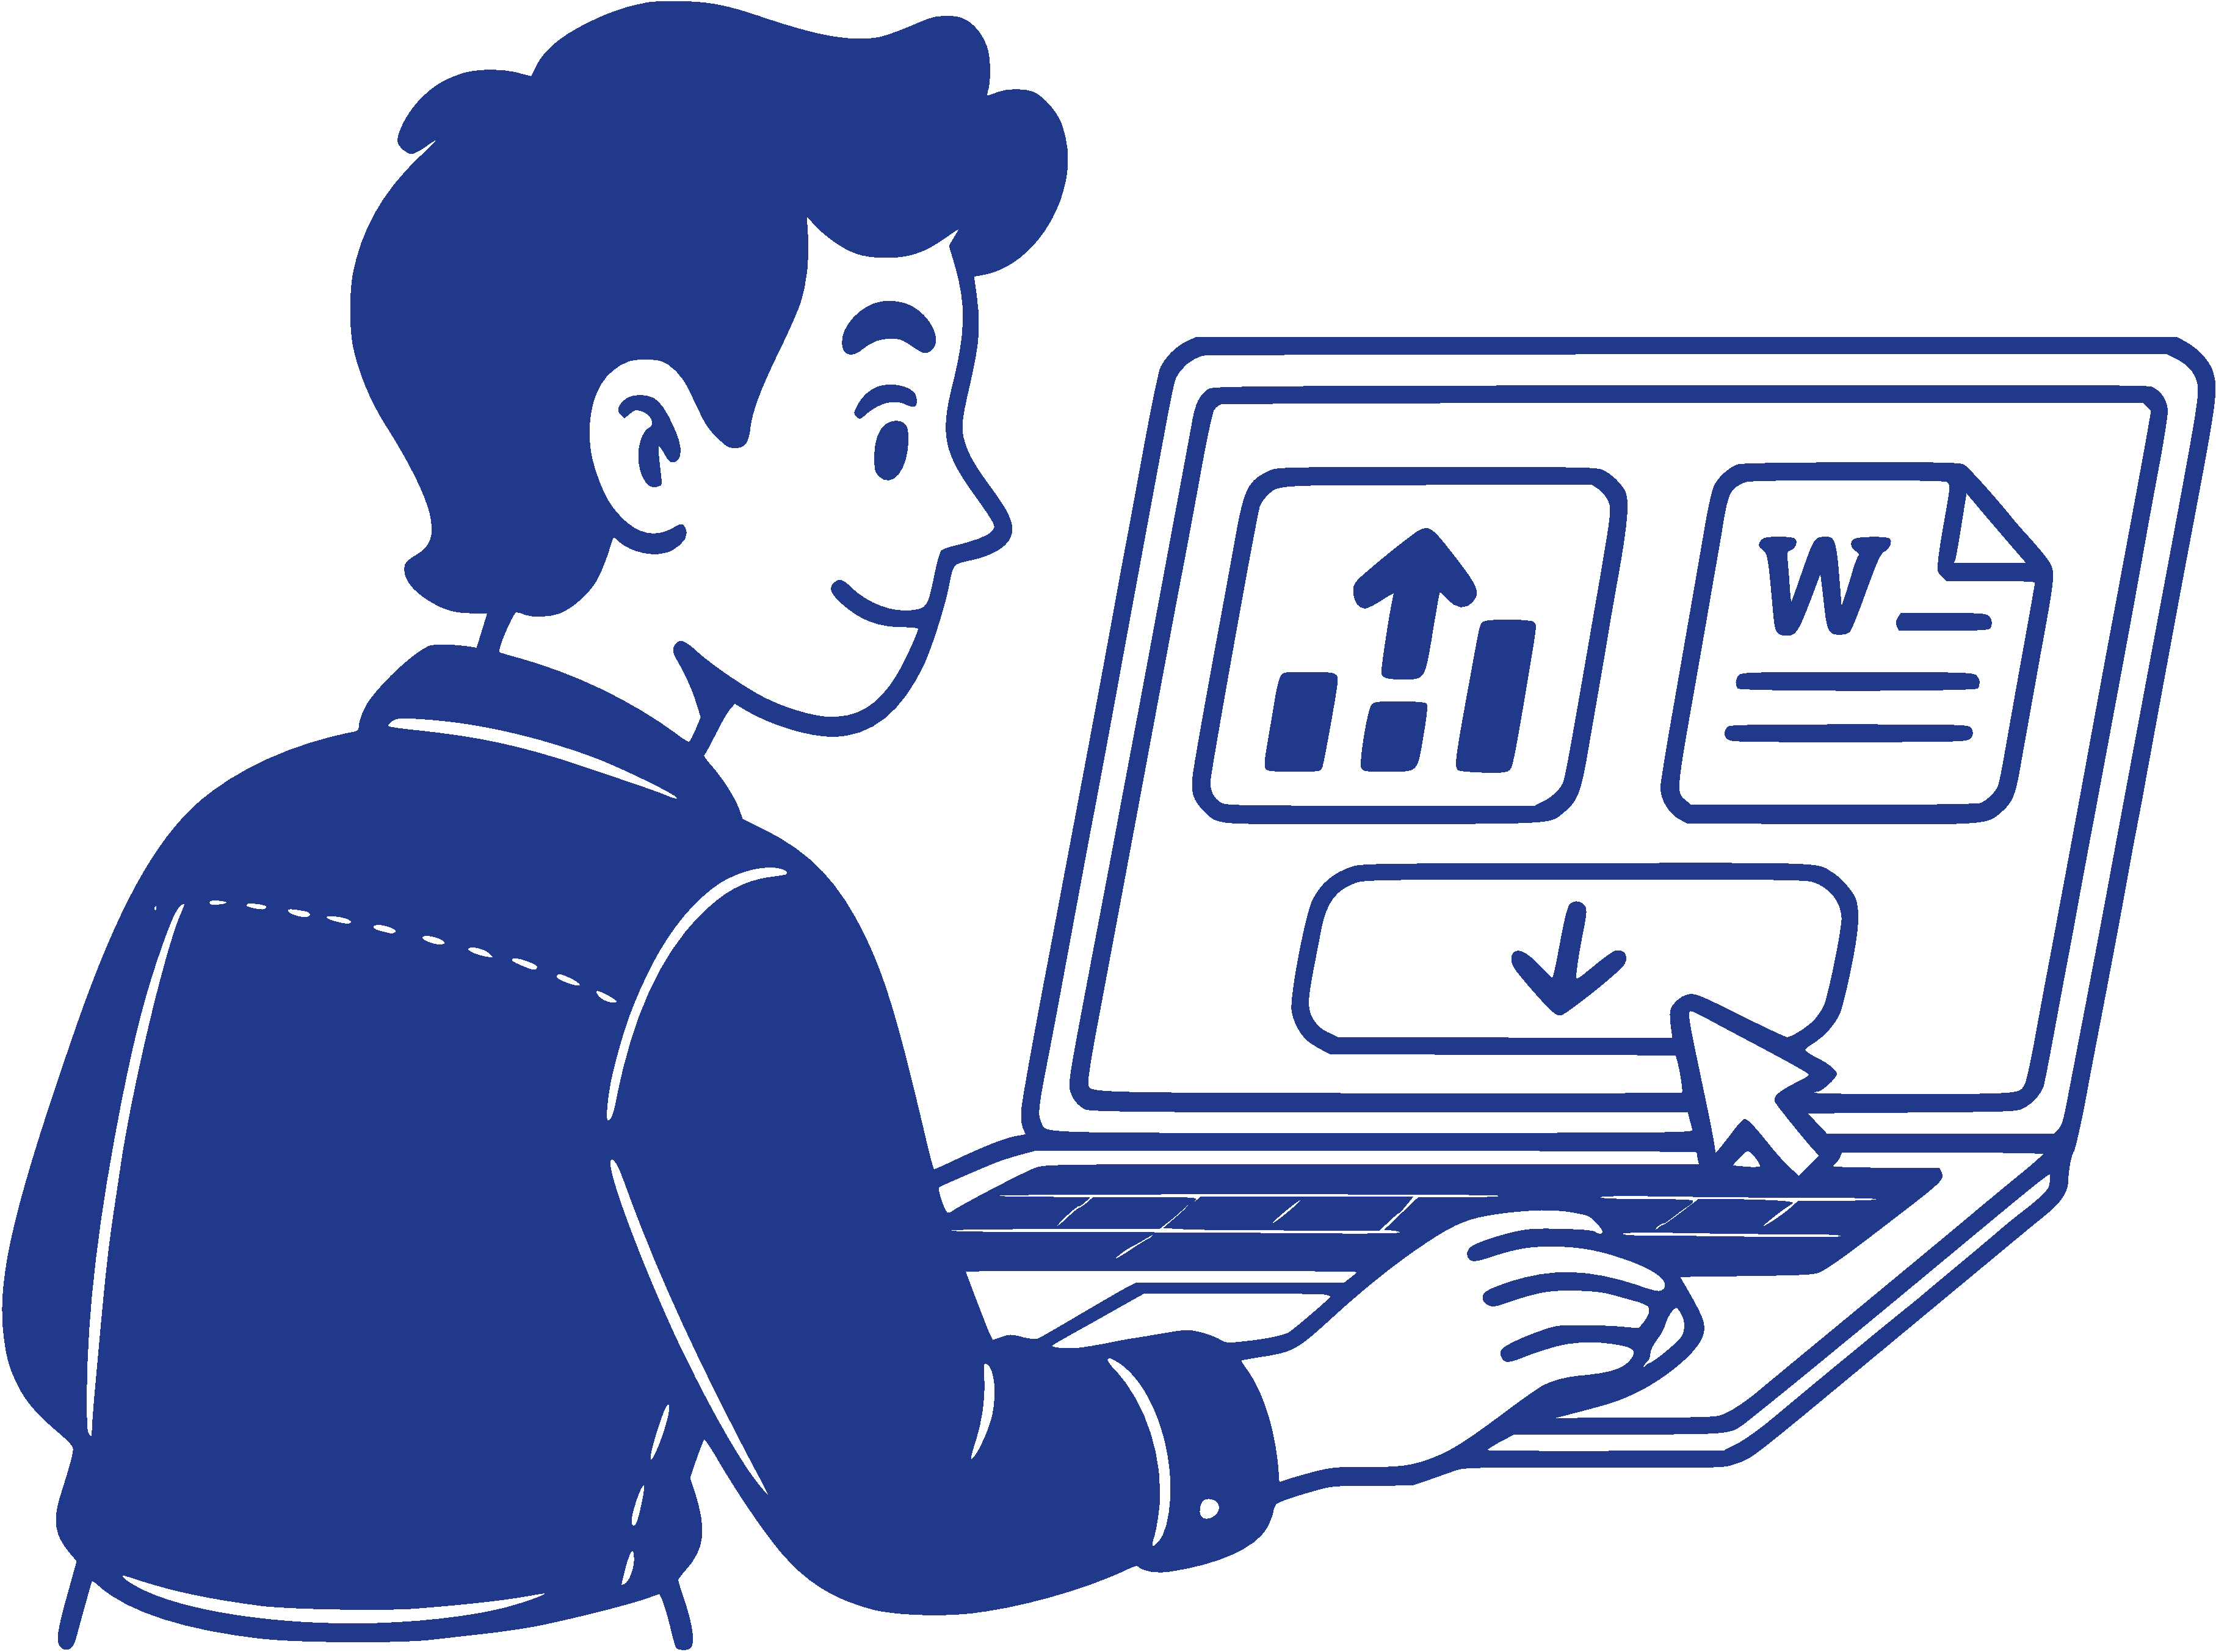
\includegraphics[width=.9\textwidth]{usage.pdf}
					\caption{Easy Usage}
				\end{figure}
			\end{column}

			\begin{column}{.65\textwidth}
				\begin{itemize}
					\item Upload templates and data
					\item Auto-fill variables and generate charts
					\item Preview and export \texttt{.docx} reports
				\end{itemize}
			\end{column}
		\end{columns}
	\end{frame}
	
	\begin{frame}{How It Works: Tools \& Technologies}
		\begin{itemize}
		  \item Backend: Python (Flask) + Pandas + DocxTpl
		  \item Frontend: HTML + JavaScript + Google Picker API
		  \item Visualization: Plotly + Kaleido
		  \item Deployment: Render with OAuth and cloud integration
		\end{itemize}
	\end{frame}

	\section{Project Overview}

\begin{frame}[fragile]{Directory Structure}
	\scriptsize
	\dirtree{%
		.1 /..
		.2 Procfile \DTcomment{Render deployment}.
		.2 README.md \DTcomment{Project overview}.
		.2 app.py \DTcomment{Flask backend}.
		.2 credentials.json \DTcomment{OAuth token}.
		.2 fonts.
		.3 cwTeXQYuan-Medium.ttf.
		.2 requirements.txt \DTcomment{Python dependencies}.
		.2 static.
		.3 app-logo-no-text.svg.
		.3 autocomplete.min.js.
		.3 favicon.ico.
		.3 main.js \DTcomment{Frontend logic}.
		.3 math.min.js.
		.3 picker.js \DTcomment{Google Drive Picker}.
		.3 style.css.
		.2 templates.
		.3 home.html.
		.3 index.html \DTcomment{Upload page}.
		.3 preview.html \DTcomment{Live preview}.
	}
	\end{frame}
	

	\begin{frame}{Step-by-Step Logic Flow}
		\begin{figure}[H]
			\centering
			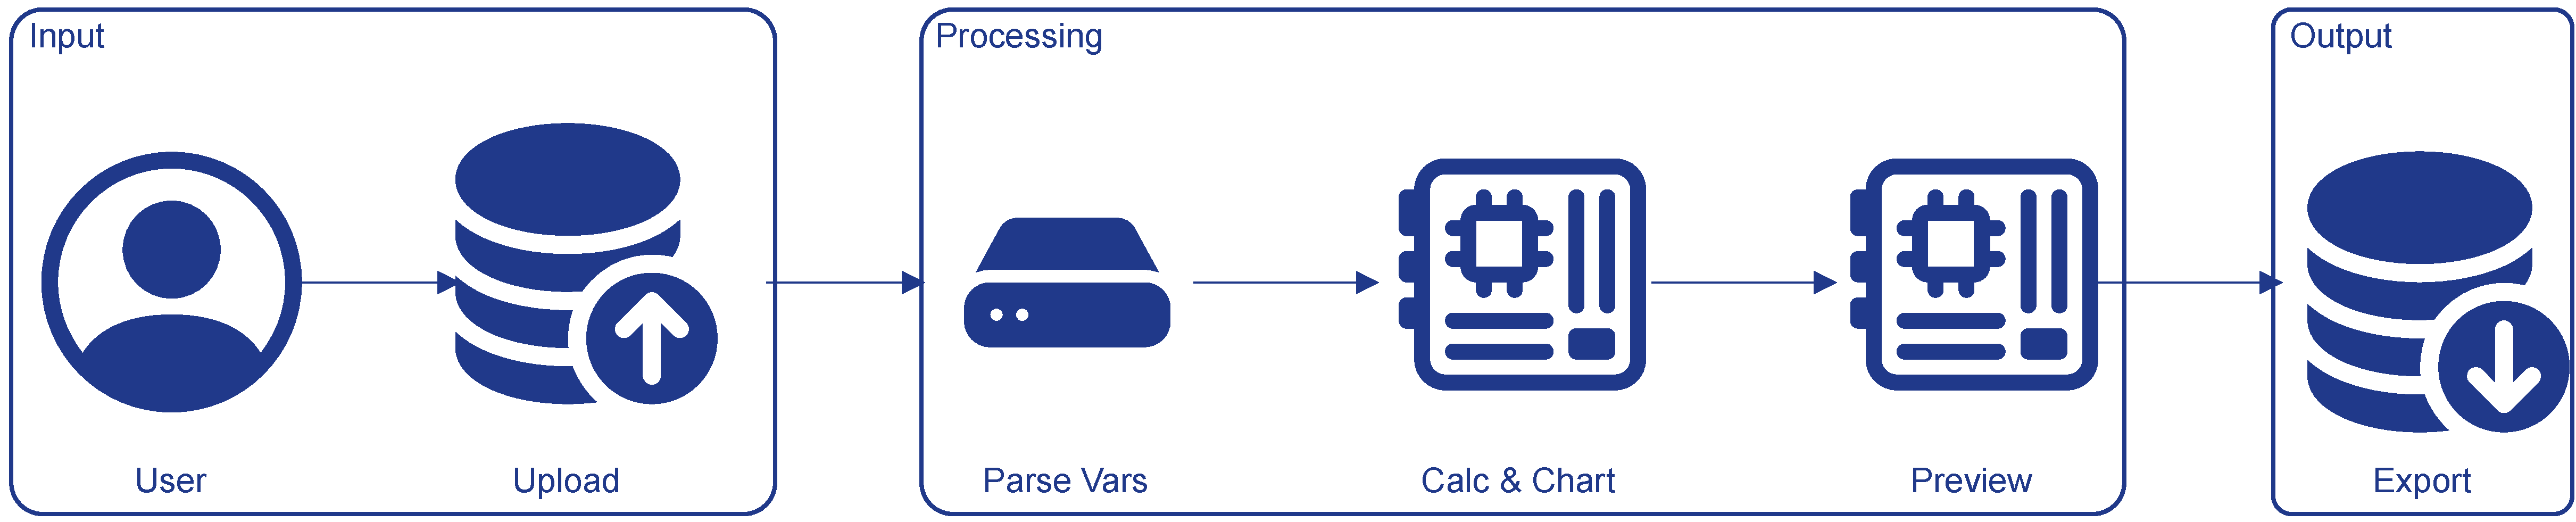
\includegraphics[width=\textwidth]{reportGen-logic.pdf}
			\caption{Report Generator Logic}
		\end{figure}
	\end{frame}

	\begin{frame}{Frontend: HTML + JS}
		\begin{itemize}
			\item Upload templates and data files
			\item Display variable previews and chart selectors
			\item Integrate \href{https://developers.google.com/workspace/drive/picker/guides/overview}{\textbf{Google Picker}} for cloud storage access
		  \end{itemize}
	\end{frame}

	\begin{frame}{Backend: Flask}
		\begin{itemize}
			\item Parse placeholders in Word templates
			\item Process formulas using data from CSV/JSON
			\item Generate and insert charts into documents
		  \end{itemize}
	\end{frame}

	\begin{frame}{Data Flow}
		\begin{enumerate}
		  \item User uploads `.docx' template and `.csv' data
		  \item Backend detects variables like \texttt{\{\{ revenue \}\}}
		  \item System evaluates formulas (e.g., \texttt{SUM(Revenue)})
		  \item Chart is generated and saved as image
		  \item Final \texttt{.docx} report is rendered and ready for download
		\end{enumerate}
	\end{frame}

	\section{Business Value}

	\begin{frame}{reportGen Can Help!}
		\begin{itemize}
			\item \textbf{Time \& Cost Saving}: Reports that took an hour now finish in minutes—saving hundreds of hours yearly across teams.
			
			\item \textbf{Reusable Templates}: Create once, reuse forever. Perfect for recurring reports with different data.
			
			\item \textbf{Fewer Errors}: Auto formulas and data validation reduce mistakes and improve consistency.
			
			\item \textbf{Cloud Ready}: Integrated with Google Drive and OAuth—easy for remote and team-based work.
		\end{itemize}
	\end{frame}

	\section{Features}

	\begin{frame}{Word Templating with Placeholders}
		\begin{itemize}
		  \item ReportGen allows users to design Word templates using placeholders such as \texttt{\{\{ total\_sales \}\}}
		  \item These placeholders are detected and replaced with values dynamically derived from uploaded datasets
		  \item Supports both scalar values and images (charts)
		\end{itemize}
	\end{frame}

	\begin{frame}{Data Upload and Variable Detection}
		\begin{itemize}
		  \item Supports CSV/Excel upload with drag-and-drop or Google Picker
		  \item Automatically detects time columns and converts them to pandas datetime
		  \item Variables in templates are cross-checked against uploaded data columns
		\end{itemize}
	\end{frame}

	\begin{frame}{Formula Engine}
		\begin{itemize}
		  \item Users can define formulas like \texttt{SUM(Sales)}, \texttt{MEAN(Revenue)}, or \texttt{PERCENT\_CHANGE(Profit)}
		  \item Formulas support chaining and nested calculations
		  \item Dependencies between variables are resolved using topological sorting to ensure correct evaluation order
		\end{itemize}
	\end{frame}

	\begin{frame}{Dynamic Chart Generation}
		\begin{itemize}
		  \item Chart types supported: Line, Bar, Pie, and Histogram
		  \item Charts are rendered using Plotly and exported as PNG via Kaleido
		  \item Charts are then inserted into the Word document at predefined placeholders
		\end{itemize}
	\end{frame}

	\begin{frame}{Real-Time Document Preview}
		\begin{itemize}
		  \item Users can preview the rendered document before downloading it
		  \item Variables with missing values are highlighted for user correction
		  \item Interactive tooltips provide variable descriptions and chart information
		\end{itemize}
	\end{frame}

	\begin{frame}{Google Drive Integration}
		\begin{itemize}
		  \item Integrated with Google Picker API for file selection from Google Drive
		  \item OAuth 2.0 authorization ensures secure access
		  \item Files selected via Google Picker are loaded directly into the website
		\end{itemize}
	\end{frame}

	\section{Implementation Details}

	\begin{frame}{Flask: Lightweight, Powerful, Modular}
		\begin{itemize}
		  \item Routes handle file uploads, previews, and report generation
		  \item Uses Jinja2 templates for dynamic HTML rendering
		  \item Session-based design to manage files and variable states per user
		\end{itemize}
	\end{frame}
	
	\begin{frame}[fragile]{Handling Requests the Flask Way}
		\begin{lstlisting}[language=Python, breaklines=true, basicstyle=\fontsize{6.5pt}{7.8pt}\selectfont]
from flask import Flask, request, render_template, redirect, url_for
app = Flask(__name__)

@app.route('/')
def home():
    return render_template('index.html')

@app.route('/submit', methods=['POST'])
def submit():
    data = request.form.get('data_field')
    return f"You submitted: {data}"

@app.route('/redirect-example')
def go_somewhere():
    return redirect(url_for('home'))

if __name__ == '__main__':
    app.run(debug=True)
\end{lstlisting}
	\end{frame}

	\begin{frame}{Template Rendering: \texttt{docxtpl}}
		\begin{itemize}
		  \item Word templates use \texttt{docxtpl} to render values into placeholders
		  \item Scalar variables (e.g., total\_sales) and charts (as images) are inserted dynamically
		  \item Charts are saved as images and embedded using InlineImage
		\end{itemize}
	\end{frame}

	\begin{frame}[fragile]{Handling Requests the Flask Way}
		\begin{lstlisting}[language=Python, breaklines=true, basicstyle=\fontsize{6.5pt}{7.8pt}\selectfont]
from docxtpl import DocxTemplate, InlineImage
from docx.shared import Mm

# Load Word template
doc = DocxTemplate("template.docx")

# Prepare image and data
chart_img = InlineImage(doc, "chart.png", width=Mm(80))
context = {
    "title": "Monthly Sales Report",
    "chart": chart_img
}

# Render and export
doc.render(context)
doc.save("output.docx")
\end{lstlisting}
	\end{frame}

	\begin{frame}{Chart Rendering: Plotly + Kaleido}
		\begin{itemize}
		  \item Charts are generated using Plotly based on user-selected configurations
		  \item The Kaleido engine converts Plotly figures to static PNG files
		  \item Chart files are inserted into Word at specified placeholders
		\end{itemize}
	\end{frame}

	\begin{frame}[fragile]{Generating Line Chart with Plotly}
		\begin{lstlisting}[language=Python, breaklines=true, basicstyle=\fontsize{6.5pt}{7.8pt}\selectfont]
import pandas as pd
import plotly.express as px

# Load data
df = pd.read_csv("sales_data.csv")

# Generate line chart
fig = px.line(
    df,
    x="date",
    y="sales",
    title="Monthly Sales Trend",
    labels={"date": "Date", "sales": "Sales Amount"}
)

# Export as PNG using Kaleido
fig.write_image("chart.png", engine="kaleido")
\end{lstlisting}
		\end{frame}
		

	\begin{frame}{Formula Parsing and Evaluation}
		\begin{itemize}
		  \item Users can define formulas in settings or interactively.
		  \item The parser supports nested formulas, dependencies, and chained evaluations.
		  \item Topological sorting ensures correct evaluation order.
		\end{itemize}
	\end{frame}

	\begin{frame}[fragile]{Formula Evaluation Example}
		\begin{lstlisting}[language=Python, breaklines=true, basicstyle=\fontsize{6.5pt}{7.8pt}\selectfont]
import pandas as pd

# Sample dataset
df = pd.DataFrame({
    'sales': [100, 200, 300],
    'cost': [30, 80, 100],
})

# Evaluate 'profit' and 'profit_margin'
context = {}
context['profit'] = (df['sales'] - df['cost']).sum()
context['profit_margin'] = context['profit'] / df['sales'].sum()
\end{lstlisting}
	\end{frame}

	\begin{frame}[fragile]{Topological Sorting \& Calculation}
		\begin{lstlisting}[language=Python, breaklines=true, basicstyle=\fontsize{6.5pt}{7.8pt}\selectfont]
# Assuming topologically sorted order
ordered_vars = ['profit', 'profit_margin', 'summary']

# Final variable using previously computed results
context['summary'] = context['profit']  # Already summed above

print(context)
# {
#   'profit': 390,
#   'profit_margin': 0.65,
#   'summary': 390
# }
\end{lstlisting}
	\end{frame}
		
	\begin{frame}{Google Picker API Integration}
		\begin{itemize}
		  \item Users can connect to their Google Drive to import `.docx`, `.csv`, and `.json` files
		  \item Authentication is handled via OAuth 2.0 with secure token storage
		  \item Picker interface allows real-time browsing of personal Drive folders
		\end{itemize}
	\end{frame}

	\begin{frame}[fragile]{Google OAuth 2.0 Integration}
		\begin{lstlisting}[language=Python, breaklines=true, basicstyle=\fontsize{6.5pt}{7.8pt}\selectfont]
from flask import Flask, redirect, session, request, url_for
from google_auth_oauthlib.flow import Flow

@app.route('/authorize')
def authorize():
    flow = Flow.from_client_secrets_file(
        'credentials.json',
        scopes=['https://www.googleapis.com/auth/drive.readonly'],
        redirect_uri=url_for('oauth2callback', _external=True)
    )
    auth_url, state = flow.authorization_url(prompt='consent')
    session['state'] = state
    return redirect(auth_url)
\end{lstlisting}
	\end{frame}

	\begin{frame}[fragile]{Handling Callback and Picker Token}
		\begin{lstlisting}[language=Python, breaklines=true, basicstyle=\fontsize{6.5pt}{7.8pt}\selectfont]
@app.route('/oauth2callback')
def oauth2callback():
    flow = Flow.from_client_secrets_file(
        'credentials.json',
        scopes=['https://www.googleapis.com/auth/drive.readonly'],
        redirect_uri=url_for('oauth2callback', _external=True)
    )
    flow.fetch_token(authorization_response=request.url)

    credentials = flow.credentials
    session['access_token'] = credentials.token

    return render_template('picker.html', token=credentials.token)
\end{lstlisting}
		\end{frame}
		
	\begin{frame}{Session Management and File Caching}
		\begin{itemize}
		  \item User uploads are stored temporarily in session-scoped folders
		  \item Word and CSV files are cached for preview reuse
		  \item On refresh, the system reuses cached content to avoid recomputation
		\end{itemize}
	\end{frame}

	\section{Conclusion}

	\begin{frame}{Project Achievements}
		\begin{itemize}
			\item Word template rendering with dynamic placeholders
			\item CSV data analysis and formula engine
			\item Chart generation and image embedding
			\item Google Drive file selection via Picker API
		\end{itemize}
	\end{frame}

	\begin{frame}{Challenges and Limitations}
		\begin{itemize}
			\item Handling \texttt{eval()} securely in a sandboxed way
			\item Limited user control over advanced chart styling
			\item Current layout is not fully responsive on mobile devices
			\item Sessions are temporary; no persistence across visits
		\end{itemize}
	\end{frame}

	\begin{frame}{Future Development Directions}
		\begin{itemize}
			\item Allow \texttt{.pdf} output with the same formatting as Word
			\item Enable login, saved reports, and version history
			\item Visual variable placement for non-technical users
			\item Let users adjust color, layout, labels before generation
			\item Shared library of reusable Word templates
		\end{itemize}
	\end{frame}

	\begin{frame}{reportGen Demonstration}
		\begin{figure}[H]
			\centering
			\includesvg[width=0.45\textwidth]{reportGen-Web}
		\end{figure}
	\end{frame}

	\begin{frame}[focus]
		\centering
		{\fontsize{30pt}{60pt}\selectfont \textbf{Q \& A}}
	  \end{frame}	  

	\begin{frame}{Feedback Form}
		\begin{figure}[H]
			\centering
			\includesvg[width=0.45\textwidth]{feedback-form}
		\end{figure}
	\end{frame}

	\begin{frame}[focus]
        \textbf{Thanks for your listening!}\\
		\vspace{10pt}
		\href{https://www.facebook.com/yueswater/}{\faIcon{facebook}}  \hspace{10pt} \href{https://github.com/xiaolong70701/reportGen}{\faIcon{github}} \hspace{10pt} \href{https://www.instagram.com/yues_19_water/}{\faIcon{instagram}}
    \end{frame}
\end{document}
